% ⚠️ 已归档 · 旧协议数据（≤2026-05）：数字来自数据泄漏协议（yolo11s.pt COCO 预训练初始化），不得用于论文或实验对比。
% 唯一可信数据源：docs/CLEAN_PROTOCOL_RESULTS.md（干净协议，2026-09-22）。归档：2026-10-08。
% ============================================
% VCP：面向小样本目标检测的单阶段余弦分类器与原型学习
% 期刊投稿论文 — 中文审阅稿
%
% Overleaf 编译设置：
%   Compiler: XeLaTeX（Menu → Compiler → XeLaTeX）
%   TeX Live:  2024 或更新
%   上传文件:  将此 .tex 文件 + 3 张 JPG 图片放在同一目录
%
% 字体说明：
%   模板要求 方正小标宋简体（标题）、黑体（章节标题）、楷体（摘要）、宋体（正文）
%   Overleaf 默认使用 Fandol 字体族（FandolSong/FandolHei/FandolKai）
%   如需严格匹配模板字体，请上传对应 .ttf/.otf 文件并取消下文注释
% ============================================

\documentclass[zihao=5,a4paper,twocolumn]{ctexart}

% ============================================
% 页面布局（CAC 2026 双栏 A4）
% ============================================
\usepackage[top=2.5cm,bottom=2.5cm,left=2cm,right=2cm,columnsep=0.8cm]{geometry}
\usepackage{indentfirst}
\setlength{\parskip}{0pt}
\setlength{\parindent}{2em}

% ============================================
% 中文字体设置（CAC 2026 模板要求）
%   标题：方正小标宋简体 20pt → \zihao{2}\biaosong
%   一级标题：黑体 小4号(12bp) 居中
%   二/三级标题：黑体 5号(10.5bp)
%   摘要：楷体 5号
%   正文：宋体 5号
%   参考文献：宋体 小5号(9bp)
%
%   若 Overleaf 上缺少下述字体，ctex 自动回退到 Fandol 字体族
%   （FandolSong → 宋体，FandolHei → 黑体，FandolKai → 楷体）
%   如需严格匹配模板，请上传字体文件并取消下方注释
% ============================================

% 方正小标宋简体（标题专用，需自行上传字体文件至 Overleaf）
% \setCJKfamilyfont{zhbiaosong}{FZXiaoBiaoSong-B05S}
% \newcommand{\biaosong}{\CJKfamily{zhbiaosong}}
% 回退：用黑体加粗近似
\newcommand{\biaosong}{\heiti}

% 章节标题格式
\CTEXsetup[format={\zihao{-4}\bfseries\centering},beforeskip={6pt},afterskip={6pt}]{section}
\CTEXsetup[format={\zihao{5}\bfseries},beforeskip={3pt},afterskip={3pt}]{subsection}
\CTEXsetup[format={\zihao{5}\bfseries}]{subsubsection}

% ============================================
% 基础包
% ============================================
\usepackage{amsmath,amssymb,amsfonts}
\usepackage{graphicx}
\usepackage{booktabs}
\usepackage{multirow}
\usepackage{cite}
\usepackage{hyperref}
\usepackage{caption}
\usepackage{abstract}
\usepackage{stfloats}

% ============================================
% 图表标题格式（五号宋体加粗）
% ============================================
\DeclareCaptionFont{wuhao}{\zihao{5}\bfseries}
\captionsetup{font=wuhao,labelsep=quad}

% ============================================
% 摘要/关键词环境（楷体 5号）
% ============================================
\renewcommand{\abstractnamefont}{\zihao{5}\heiti}
\renewcommand{\abstracttextfont}{\zihao{5}\kaishu}
\setlength{\abstitleskip}{-0.5em}

\newenvironment{keywords}{\par\noindent\zihao{5}\heiti 关键词：}{\par}

% ============================================
% 页眉页脚（简洁风格）
% ============================================
\usepackage{fancyhdr}
\pagestyle{fancy}
\fancyhf{}
\fancyhead[L]{\zihao{-5}\songti 2026中国自动化大会（CAC 2026）}
\fancyhead[R]{\zihao{-5}\songti 费祥：VCP——面向小样本目标检测的单阶段余弦分类器与原型学习}
\fancyfoot[C]{\zihao{-5}\thepage}
\renewcommand{\headrulewidth}{0.4pt}

% ============================================
% 标题格式（CAC 2026：方正小标宋简体 20pt，段前6pt 段后6pt）
% ============================================
\makeatletter
\def\@maketitle{%
  \newpage
  \begin{center}%
    \vspace*{6pt}%
    {\fontsize{20pt}{28pt}\selectfont\biaosong\bfseries\@title\par}%
    \vskip 6pt%
    {\zihao{5}\kaishu\@author\par}%
    \vskip 2pt%
  \end{center}%
}
\makeatother

% ============================================
\begin{document}

% --- 标题 ---
\title{VCP：面向小样本目标检测的单阶段余弦分类器与原型学习}

% --- 作者 ---
\author{费祥\\[2pt]
\zihao{-5}\songti 曲阜师范大学~~工学院，山东~~日照~~276826}

\maketitle

% ============================================
% 摘要
% ============================================
\begin{abstract}
小样本目标检测（Few-Shot Object Detection, FSOD）旨在利用少量标注样本检测新类别，现有方法几乎全部基于两阶段检测器Faster R-CNN，而工业部署中占主导的YOLO系列单阶段检测器在FSOD场景下缺乏系统性研究。本文提出VCP框架，在TFA协议下首次将单阶段YOLO检测器与余弦分类头及原型学习相结合，构建面向FSOD的单阶段检测框架。在PASCAL VOC数据集上，VCP以仅9.5M参数的YOLO11s在10-shot设定下达到72.2\% mAP50（三划分均值），以约1/6参数量达到与两阶段SOTA方法competitive的性能；5-shot下三划分均值为58.1\%，余弦分类器相对标准微调提升达+24.7个百分点。然而在COCO数据集上，同样的余弦分类器策略反而不如标准微调基线。通过系统的Precision-Recall分解分析（24组对比），本文揭示了余弦分类器本质上是一个召回率增强器（Recall Booster）——在所有shot和数据集上一致地将工作点推向高召回、低精确方向。其最终收益方向取决于基线召回率提升空间与数据集P-R权衡比的乘积效应：VOC同时具备低基线召回率与有利权衡比，收益显著；COCO面临不利权衡比，精确率损失压倒召回增益。此外，本文探索了Florence-2视觉语言模型（VLM）语义原型作为辅助先验，在10-shot下三个划分均带来正向增量（均值+0.5 pp），方向一致但幅度有限，其零样本扩展潜力值得进一步研究。这一工作为理解单阶段FSOD中分类器行为提供了新的分析视角。
\end{abstract}

\begin{keywords}
小样本目标检测；单阶段检测器；余弦分类器；原型学习；召回率增强
\end{keywords}

% ============================================
% 1 引言
% ============================================

\section{引言}

小样本目标检测旨在从少量标注样本中学习检测新类别的能力，是计算机视觉领域兼具理论价值和实际应用需求的研究方向。近年来，以FSCE~\cite{sun2021fsce}、DeFRCN~\cite{qiao2021defrcn}为代表的方法取得了显著进展，在PASCAL VOC和COCO等基准数据集上持续刷新性能记录。

然而，现有FSOD方法存在一个显著的共性：几乎全部基于两阶段检测器Faster R-CNN~\cite{ren2015faster}。这一范式选择具有历史原因——Faster R-CNN的区域提议网络（RPN）天然提供了前景筛选机制，在小样本场景下有助于控制假阳性。但在工业部署和实际应用中，YOLO系列~\cite{redmon2016yolo,jocher2023ultralytics}单阶段检测器以其高效率和实时性占据绝对主导。FSOD研究社区对单阶段检测器的忽视，导致了"论文方法用不上、实际部署没人研究"的尴尬局面。据我们所知，在TFA标准协议下，尚未有工作系统研究现代YOLO检测器（YOLOv8及以上）在FSOD中的表现。

单阶段检测器在FSOD中面临的核心挑战在于缺乏独立的RPN前景筛选：在没有足够训练样本的情况下，密集预测范式容易产生大量低质量候选框，导致分类器面临极高的正负样本不平衡。近年来，余弦分类头~\cite{wang2020tfa}在FSOD中被广泛采用，其归一化特性有助于缓解小样本下的分类器过拟合。与此同时，Florence-2~\cite{xiao2024florence2}等视觉语言模型展现了强大的语义理解能力。然而，将余弦分类头与单阶段YOLO检测器结合，并系统分析其在小样本场景下的行为特性，目前仍是空白。

本文提出VCP（Visual-Cosine-Prototype），在TFA协议下构建了面向FSOD的单阶段检测框架。VCP以YOLO11s为基础检测器，将其线性分类头替换为余弦相似度分类器，利用支持集视觉特征构造类别原型（Proto模式），并探索了Florence-2语义描述作为辅助先验的融合方案（Fused模式）。在PASCAL VOC数据集上，VCP展现出具有竞争力的性能（见表1）：10-shot三划分均值达72.2\% mAP50，以仅约9.5M参数达到与基于60M参数Faster R-CNN R-101的SOTA方法competitive的水平，其中Split 1达74.7\%，超越了已有方法。3-shot和5-shot下同样取得有竞争力的结果。

然而，当我们将同样的方法应用于COCO数据集时，却观察到了截然相反的现象：余弦分类器系列方法在COCO上全面落后于标准微调基线。通过系统的Precision-Recall分解分析，我们识别出余弦分类器的一致行为模式：

\begin{itemize}
\item 余弦分类器在两个数据集上呈现一致的行为模式——在所有shot设定下无一例外地牺牲精确率换取召回率，可被定性为"召回率增强器"（Recall Booster）；
\item 差异来自数据集的P-R权衡比（Tradeoff Ratio）：VOC上每单位召回增益仅需付出较小的精确率代价，召回增益主导最终结果；而COCO上类别数多（20 vs 5）、场景复杂，余弦分类器的宽松决策边界在更多类别间产生大量交叉假阳性，精确率损失主导了最终性能。
\end{itemize}

基于以上观察，本文提出"P-R权衡假说"（P-R Tradeoff Hypothesis）：余弦分类器天然地将检测器推向高召回、低精确的工作点，其最终收益方向取决于基线召回率提升空间与数据集P-R权衡比的乘积效应——VOC同时具备低基线召回率与有利权衡比，收益显著；COCO面临不利权衡比，精确率损失压倒召回增益。

本文的主要贡献包括：（1）在TFA协议下首次系统探索了单阶段YOLO检测器在FSOD中的可行性，以1/6参数量达到competitive性能；（2）通过24组P-R分解识别出余弦分类器作为Recall Booster的一致行为模式，为理解单阶段FSOD中分类器行为提供了分析框架；（3）初步探索了VLM语义原型作为辅助先验的价值与局限。

% ============================================
% 2 相关工作
% ============================================

\section{相关工作}

\subsection{小样本目标检测}

小样本目标检测的研究范式主要分为两类：基于元学习的方法和基于微调的方法。早期工作如Meta R-CNN~\cite{yan2019meta}、MetaDet~\cite{wang2019meta}采用元学习策略，通过在基类和新类任务间交替训练来学习跨类别泛化能力。TFA~\cite{wang2020tfa}（Two-stage Fine-tuning Approach）首次系统地论证了简单的两阶段微调策略即可超越复杂的元学习方法，将FSOD简化为：第一阶段在基类上训练检测器，第二阶段在新类上微调分类头。此后，大量工作沿袭TFA的微调范式并加以改进。

FSCE~\cite{sun2021fsce}提出对比提议编码损失（Contrastive Proposal Encoding Loss），通过增强候选框特征的类内紧凑性和类间可分性来改善余弦分类器的判别能力。DeFRCN~\cite{qiao2021defrcn}从梯度优化的角度出发，提出梯度解耦层（Gradient Decoupled Layer），对RPN、分类头和回归头施加不同的梯度缩放因子，缓解了小样本下骨干网络过拟合的问题。KD-DeFRCN~\cite{pei2022kddefrcn}进一步引入知识蒸馏，将基类模型的知识迁移到新类分类头。此外，MPSR~\cite{wu2020mpsr}、FSDetView~\cite{xiao2020fsdetview}、CME~\cite{li2021cme}等方法从多尺度特征、视角增强、上下文建模等角度对FSOD进行了改进。

上述方法虽然在技术路径上各有差异，但共享一个共同的基础检测器：Faster R-CNN。这一现象并非偶然——RPN的前景筛选机制为小样本场景提供了天然的候选框质量控制，而单阶段检测器因其密集预测特性，在小样本下容易陷入严重的正负样本失衡。然而，近年来的技术进展——包括余弦分类头的归一化能力、VLM提供的语义先验、以及YOLO系列检测头设计的成熟——使得重新审视单阶段FSOD成为可能。

\subsection{单阶段检测器及其在FSOD中的探索}

YOLO系列检测器自YOLOv1~\cite{redmon2016yolo}以来经历了持续迭代。从YOLOv3~\cite{redmon2018yolov3}引入FPN多尺度特征融合，到YOLOv5/YOLOv8的解耦检测头（Decoupled Head）设计，再到YOLOv11的Anchor-Free范式，单阶段检测器的检测精度和训练稳定性已今非昔比。这些架构演进为单阶段检测器处理小样本场景奠定了基础：解耦头使得分类和定位可以独立优化，Anchor-Free设计减少了预设超参数对稀有类别的偏差，而更深的骨干网络提供了更丰富的特征表示。

然而，FSOD社区对单阶段检测器的探索极为有限。Meta-YOLO~\cite{kang2019fsrw}是较早的尝试，通过元学习中的特征调制机制（Feature Modulation）将支持集信息注入YOLOv2检测器。但该方法采用的是Kang等人提出的数据划分协议~\cite{kang2019fsrw}，该协议因随机种子高方差问题已被后续工作普遍弃用，转向TFA提出的低方差划分协议~\cite{wang2020tfa}。在TFA协议下，尚未有工作系统研究现代YOLO检测器（YOLOv8及以上）在FSOD中的表现，更遑论结合VLM原型与余弦分类头。

\subsection{视觉语言模型在检测中的应用}

CLIP~\cite{radford2021clip}通过4亿图文对的大规模对比预训练，首次展示了VLM强大的零样本图像识别能力，其文本编码器能够为任意自然语言描述的类别生成语义嵌入。这一范式为FSOD中的原型构造提供了重要启发——传统FSOD方法需要从少量训练样本中平均特征来构造类别原型，而VLM可以直接从文本描述中获取语义先验。

Florence-2~\cite{xiao2024florence2}是微软提出的新一代视觉基础模型（CVPR 2024），采用统一的多任务序列到序列架构，能够根据文本提示执行目标检测、分割、图像描述等多种视觉任务。与CLIP仅提供全局图文对齐不同，Florence-2在细粒度视觉语义方面具有更强的表征能力，尤其适合通过任务提示（如"\texttt{<DETAILED\_CAPTION>}"）为目标区域生成丰富的语义描述。本文的Fused模式即利用这一特性，将Florence-2的语义描述编码为原型补充信息，与视觉原型进行可学习融合。

在检测领域，VLM已被广泛应用于开放词汇检测（Open-Vocabulary Detection, OVD）。OWL-ViT~\cite{minderer2022owlvit}、GLIP~\cite{li2022glip}、Grounding DINO~\cite{liu2023groundingdino}等方法将VLM的语义空间与检测器对齐，实现了对任意类别的零样本检测。但这些方法面向的是开放词汇场景，训练数据和计算开销远大于FSOD设定。在FSOD的严格数据约束下——每个新类别仅有1-10个标注样本——如何有效利用VLM原型而不引入过度的语义噪声，是一个未被充分探索的问题。

% ============================================
% 3 方法
% ============================================

\section{方法}

\subsection{整体框架}

VCP的整体框架如图1所示。基础检测器采用YOLO11s，保留其骨干网络（Backbone）和颈部网络（Neck）的设计，但对检测头中的分类分支进行关键替换：将标准的线性分类层替换为余弦相似度分类器。

\begin{figure*}[t]
\centering
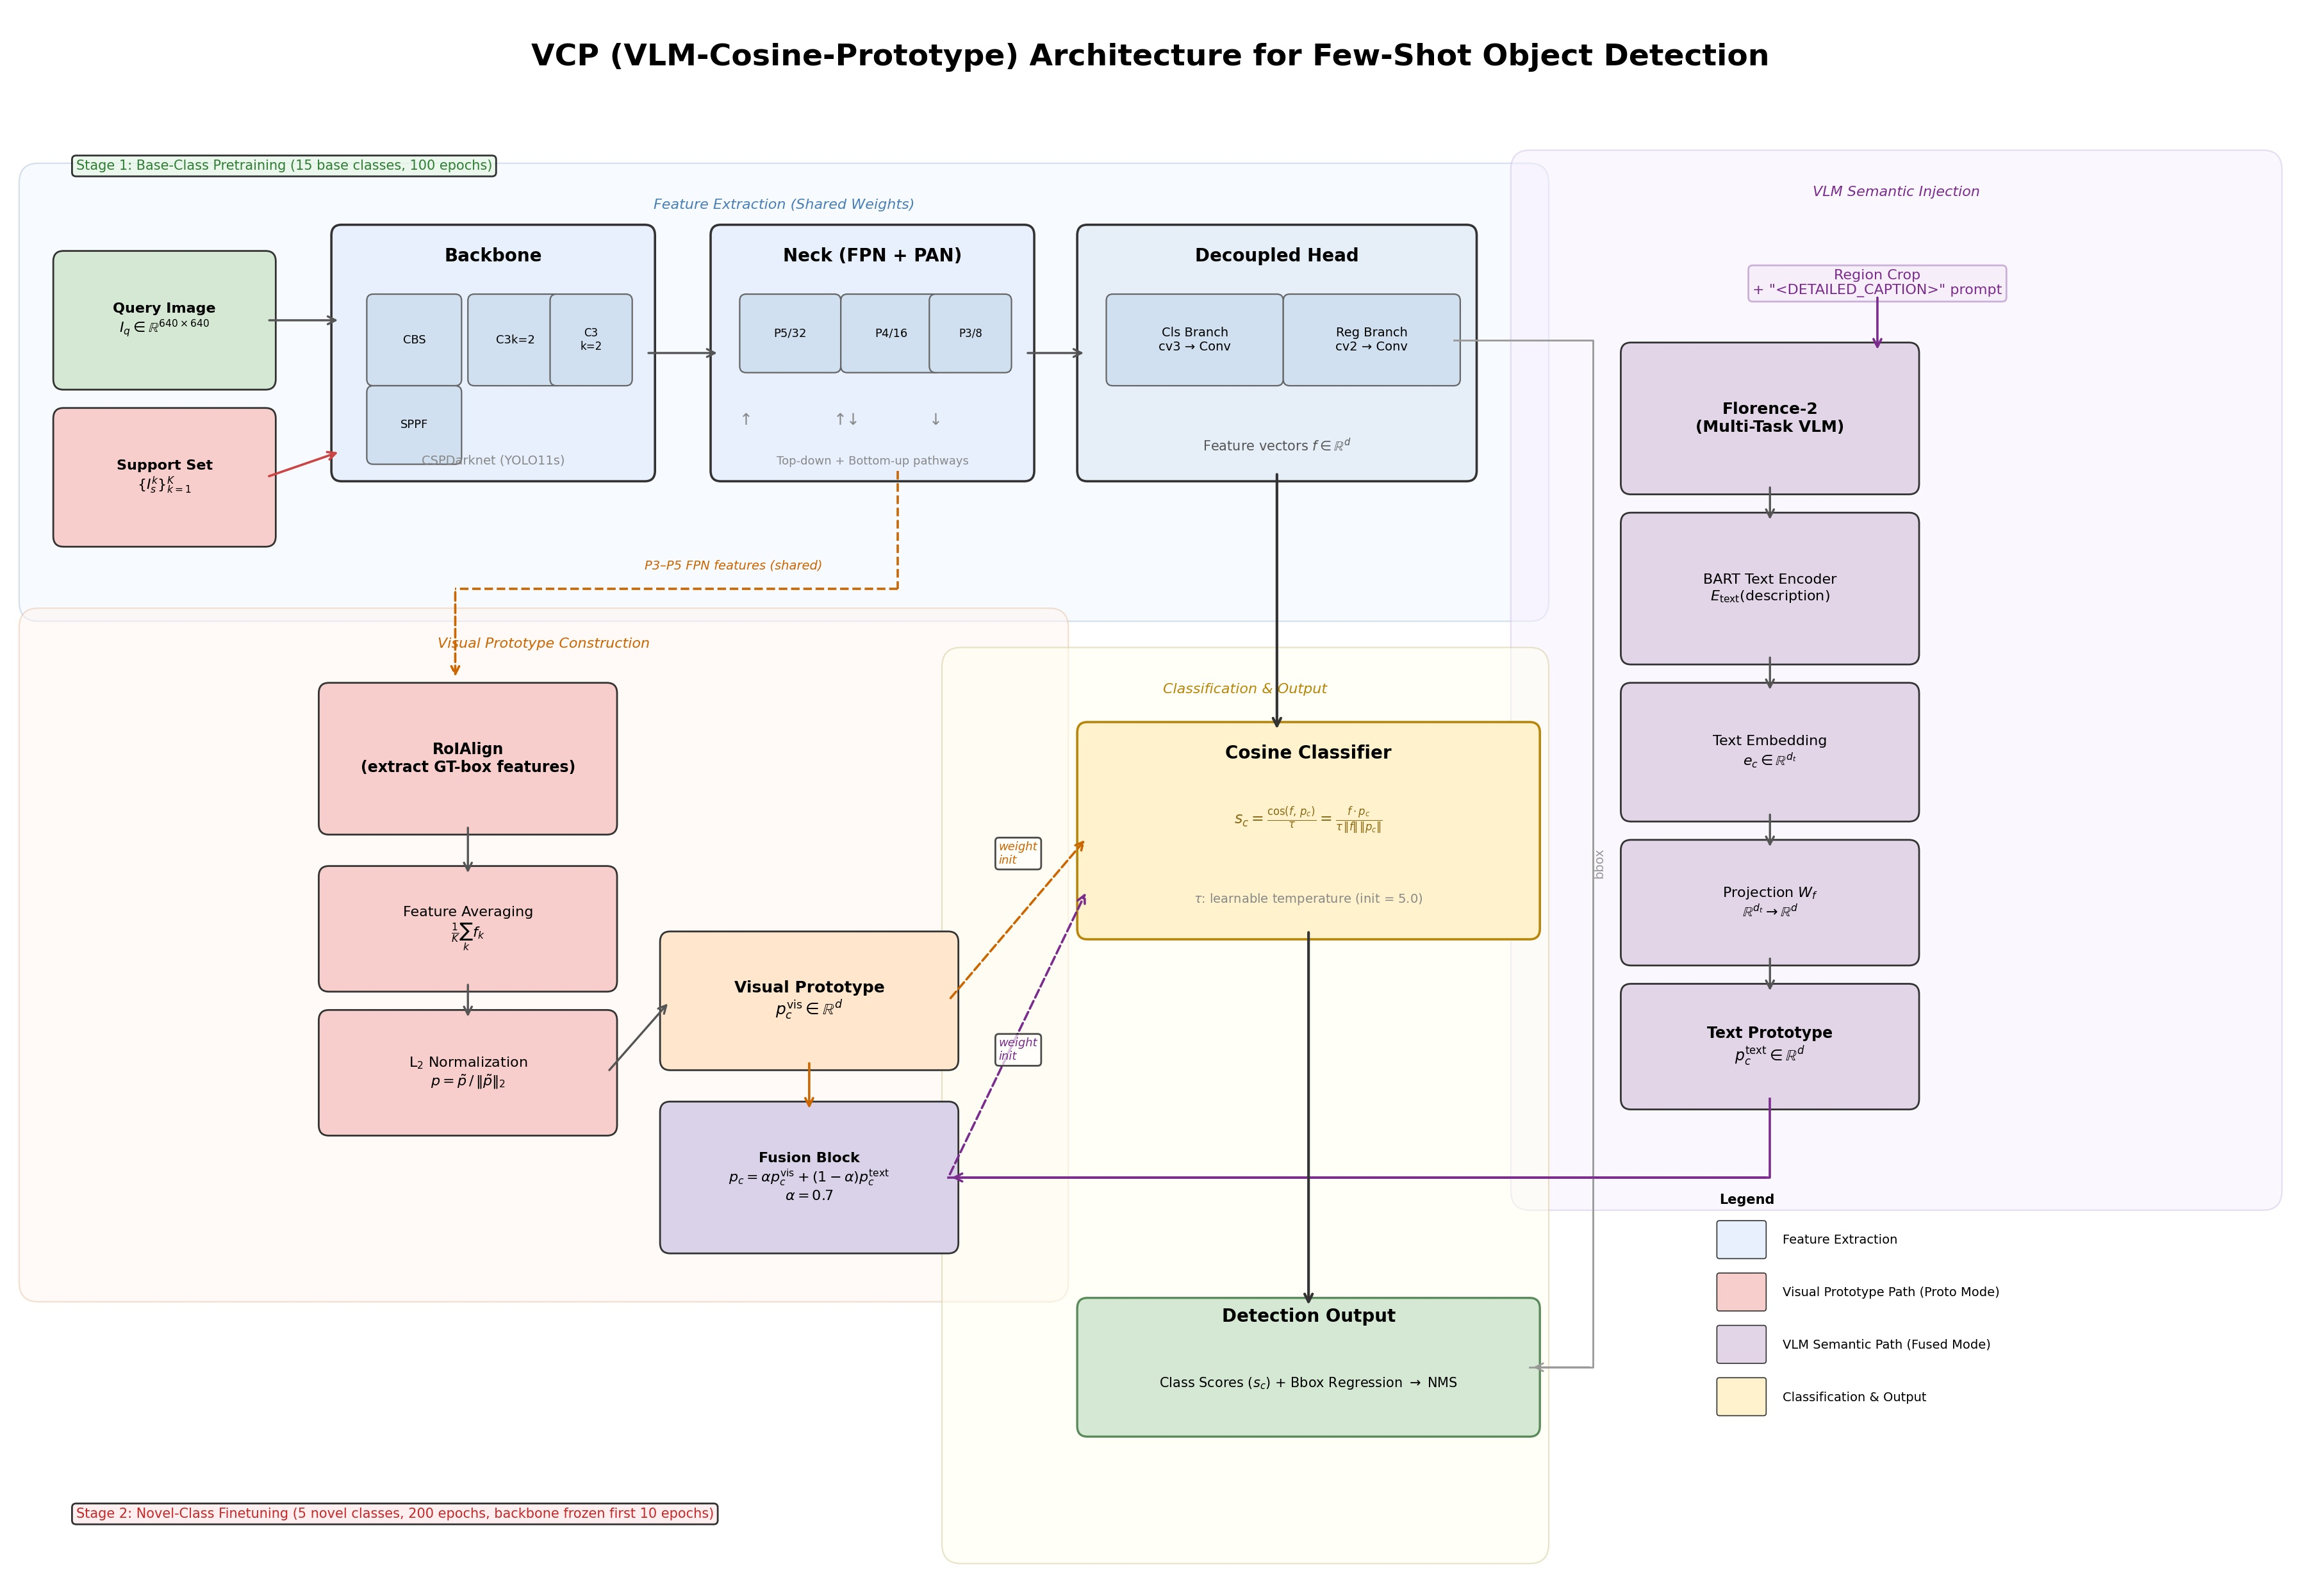
\includegraphics[width=\textwidth]{fig1_framework.jpg}
\caption{VCP整体框架图。Input：输入图像；Backbone+Neck：YOLO11s特征提取；Decoupled Head：解耦检测头；Cosine Classifier：余弦分类器；Support Set$\rightarrow$RoIAlign$\rightarrow$Visual Prototype：视觉原型提取；Florence-2$\rightarrow$BART$\rightarrow$Text Prototype：语义原型提取；Fusion：特征级融合（$\alpha=0.7$）。}
\label{fig:framework}
\end{figure*}

具体而言，对于检测头输出的每个候选框特征向量 $f \in \mathbb{R}^d$，标准YOLO分类头通过线性变换 $Wf + b$ 计算各类别的logit，其中 $W \in \mathbb{R}^{C \times d}$ 为分类权重矩阵。VCP将其替换为余弦相似度计算：

\begin{equation}
s_c = \frac{\cos(f, p_c)}{\tau} = \frac{f \cdot p_c}{\tau \cdot \|f\| \cdot \|p_c\|}
\label{eq:cosine}
\end{equation}

其中 $p_c$ 为第 $c$ 类的原型向量，$\tau$ 为温度系数，控制分类概率分布的锐度。余弦分类头的归一化特性（$\|f\| = \|p_c\| = 1$）使得分类决策仅依赖于方向一致性而非向量模长，有效缓解了小样本场景下的分类器过拟合问题。

\subsection{视觉原型提取与VLM语义注入}

VCP的原型构造包含两个互补的来源：来自支持集的视觉原型和来自Florence-2的语义原型。

\textbf{视觉原型提取}：对于每个新类别 $c$，将其 $K$ 个支持样本输入检测器，使用RoIAlign在FPN输出的P3-P5层上提取GT框内特征。取检测头分类分支的输入特征（cv3层输出）进行平均，得到该类别的视觉原型：

\begin{equation}
\tilde{p}_c^{\text{vis}} = \frac{1}{K} \sum_{i=1}^{K} \text{RoIAlign}(F_i, b_i)
\label{eq:visual_proto}
\end{equation}

其中 $F_i$ 为FPN多尺度特征，$b_i$ 为GT边界框。视觉原型经过L2归一化后可直接作为余弦分类器的初始类别向量：$p_c = \tilde{p}_c^{\text{vis}} / \|\tilde{p}_c^{\text{vis}}\|_2$。此即\textbf{Proto模式}——用少量标注样本中提取的视觉特征来锚定分类决策空间。

\textbf{Florence-2语义原型}：Florence-2是微软提出的统一视觉基础模型（CVPR 2024），采用多任务序列到序列架构。VCP利用其文本编码器（BART）为每个新类别生成语义原型。具体而言，将目标区域裁剪后以``\texttt{<DETAILED\_CAPTION>}''任务提示送入Florence-2，获取该区域的细粒度文本描述，再通过BART编码器得到语义嵌入向量。视觉原型与Florence-2语义原型以可学习的融合权重 $\alpha$ 进行加权（默认 $\alpha=0.7$），实现视觉先验与语义先验的互补。此即\textbf{Fused模式}。

\subsection{原型融合策略}

VCP设计了两种原型与余弦分类器的集成模式：

\textbf{Proto模式}：利用支持集样本的视觉特征平均来初始化余弦分类头。具体而言，对每个新类别，将少量标注样本通过检测器的RoIAlign提取候选框特征，在FPN的P3-P5层上取分类分支输入特征（cv3）进行平均，L2归一化后直接写入余弦分类头的权重矩阵。此模式下，原型仅来自支持集视觉信息，分类决策完全基于视觉特征与类别原型的余弦相似度。Proto模式不依赖任何VLM，其有效性依赖于余弦分类器的归一化特性——即使少量样本的平均特征也能提供合理的类别中心估计。

\textbf{Fused模式}：在视觉原型基础上，引入Florence-2文本编码器生成的语义原型进行加权融合。余弦分类头的初始权重 $p_c$ 由视觉原型和Florence-2语义原型以可学习比例混合得到：

\begin{equation}
p_c = \alpha \cdot p_c^{\text{vis}} + (1 - \alpha) \cdot W_f \cdot p_c^{\text{text}}
\label{eq:fused}
\end{equation}

其中 $\alpha = 0.7$ 为融合权重（视觉原型占主导），$W_f$ 为可学习的投影矩阵，将Florence-2文本嵌入映射到视觉特征空间，$p_c^{\text{text}}$ 为Florence-2 BART编码器对``\texttt{<DETAILED\_CAPTION>}''任务描述文本的编码输出。

两种模式的本质区别在于知识的粒度与来源：Proto模式仅依赖支持集视觉信息，简单高效，但受限于少量样本的特征质量；Fused模式额外利用Florence-2的语义先验来修正和补充视觉原型，可能在视觉特征不可靠时（如遮挡、小目标）提供更有判别力的语义引导，但引入了额外的VLM推理开销。

\subsection{Cosine分类器的召回增强机制分析}

本节分析余弦分类器为何在FSOD中呈现"高召回、低精确"的行为特征，为第4章的实验现象提供理论基础。

考虑余弦分类器的梯度特性。对于特征向量 $f$ 和类别原型 $p_c$，余弦相似度对 $f$ 的梯度为：

\begin{equation}
\frac{\partial \cos(f, p_c)}{\partial f} = \frac{p_c - \cos(f, p_c) \cdot f}{\|f\|}
\label{eq:gradient}
\end{equation}

该梯度的关键性质在于：当 $f$ 与 $p_c$ 的相似度较低时，梯度幅值较大，更新方向朝向原型 $p_c$；当相似度已较高时，梯度幅值趋于减小。这意味着训练过程中，\textbf{低置信度的样本（通常是难例或边界样本）获得了更大的参数更新}，模型倾向于不断拓宽类别决策边界的覆盖范围。

这一梯度特性与传统线性分类器形成对比。线性分类器的梯度 $\partial (W_c f) / \partial f = W_c$ 不依赖于 $f$ 与类别中心的距离，对所有样本的更新力度均匀。因此，余弦分类器天然地偏向于"宁可错杀、不可放过"的分类策略：它可以检测出更多潜在的正确目标（高召回），但同时也会将大量背景或易混淆类别的候选框纳入（低精确）。

当视觉原型和Florence-2语义原型共同作用时，这一效应被进一步放大。Florence-2文本编码器从大规模预训练中习得的细粒度语义知识可以为类别提供更"宽松"的语义边界——例如，Florence-2可能认为"沙发"与"椅子"、"长凳"都有较高的语义关联，其语义原型在空间中处于一个更宽泛的邻域中心。这使得余弦分类器在语义原型的引导下，能够覆盖到仅靠少量训练样本无法触及的类别实例，但也同时引入了更多的类间混淆。

基于以上分析，我们提出一个可验证的假设：\textbf{视觉原型+余弦分类器的召回增强效应，其最终收益方向取决于基线召回率提升空间与数据集P-R权衡比的乘积效应}。若基线召回率低且权衡比有利（如VOC），余弦分类器带来的大幅召回提升足以抵消精确率损失，mAP显著上升；若权衡比不利（如COCO），精确率损失成为主导因素，mAP反而下降。第4.3节的实验将系统验证这一假设。

% ============================================
% 4 实验
% ============================================

\section{实验}

\subsection{实验设置}

\textbf{数据集}：采用两项FSOD标准基准——PASCAL VOC 2007+2012和MS COCO 2014。遵循TFA~\cite{wang2020tfa}的数据划分协议，VOC的20个类别随机划分为15个基类和5个新类（3个随机划分），COCO中与VOC重叠的20个类别作为新类，其余60类作为基类。评价指标采用mAP50、mAP50-95、Precision和Recall，均在PASCAL VOC 2007测试集和COCO minival上评估。

\textbf{实现细节}：基础检测器采用YOLO11s（9,458,758参数，约9.5M），预训练权重来自COCO基类训练。训练分为两个阶段：基类预训练（Stage 1）在VOC 15个基类上进行100个epoch，batch size 64，初始学习率0.01；新类微调（Stage 2）在5个新类上进行200个epoch（实际因early stopping提前终止），batch size 4，初始学习率0.0005。优化器为SGD，momentum 0.937，weight decay 0.0005，warmup 3个epoch。前10个epoch冻结backbone。数据增强包括mosaic（最后10个epoch关闭）、RandAugment、随机翻转、HSV抖动（H=0.015, S=0.7, V=0.4）、随机平移（0.1）、随机缩放（0.5）和随机擦除（probability 0.4）。图像尺寸统一为$640\times640$。Early stopping patience设为30个epoch。余弦分类头温度$\tau$初始化为5.0（可学习参数）。所有实验在单张NVIDIA H20 GPU上完成。

\textbf{基线方法}：对比四种变体——（1）Finetune：标准YOLO11s微调，线性分类头；（2）Cosine：将分类头替换为余弦分类器，权重随机初始化、通过训练学习；（3）Cosine+Proto：余弦分类头，权重由支持集视觉原型（RoIAlign特征平均）初始化；（4）Cosine+Fused：余弦分类头，权重由视觉原型与Florence-2语义原型以可学习比例融合初始化。

\subsection{主实验结果}

\textbf{PASCAL VOC结果}：表1展示了VOC数据集上四种方法在不同shot下的mAP50表现，报告Split 1结果及三划分均值±标准差。

\begin{table}[ht]
\centering
\footnotesize
\caption{VOC mAP50结果（Split 1 / 三划分均值$\pm$标准差）}
\label{tab:voc_main}
\begin{tabular}{lcccc}
\toprule
方法 & 1-shot & 3-shot & 5-shot & 10-shot \\
\midrule
Finetune      & 10.9 / --   & 20.5 / --    & 32.9 / --    & 51.3 / --     \\
Cosine        & 12.8 / --   & 51.3 / --    & 66.9 / 57.8$\pm$2.9 & 70.7 / 69.0$\pm$3.1 \\
Cosine+Proto  & 21.5 / --   & 52.3 / --    & 68.8 / 57.8$\pm$2.8 & 74.4 / 71.7$\pm$2.7 \\
Cosine+Fused  & \textbf{21.3} / -- & \textbf{53.9} / -- & \textbf{69.0} / 58.1$\pm$2.5 & \textbf{74.7} / \textbf{72.2}$\pm$2.6 \\
\bottomrule
\end{tabular}
\end{table}

从表1可以观察到三个核心趋势：（1）余弦分类器的引入带来了质的飞跃——5-shot下三划分均值从32.9\%提升至57.8\%（+24.9 pp），10-shot下从51.3\%提升至69.0\%（+17.7 pp），增益方向跨划分一致；（2）视觉原型初始化（Proto）在10-shot下带来额外+2.7 pp（三划分均值），余弦分类头与视觉原型共同贡献了绝大部分性能增益；（3）Fused模式在所有shot下均略优于Proto模式，10-shot三划分均值增益为+0.5 pp（71.7\%$\rightarrow$72.2\%），三个划分方向一致为正（+0.3/+0.7/+0.5 pp），幅度有限但体现了VLM语义先验的正向价值。VCP缩写的含义为Visual-Cosine-Prototype。

图2展示了各方法mAP50随shot数量的变化趋势，图3以Precision-Recall散点图直观呈现了余弦分类器将工作点向"高召回、低精确"方向推动的一致性行为，以及该行为在VOC和COCO上导致相反mAP结果的根本原因。

\begin{figure*}[t]
\centering
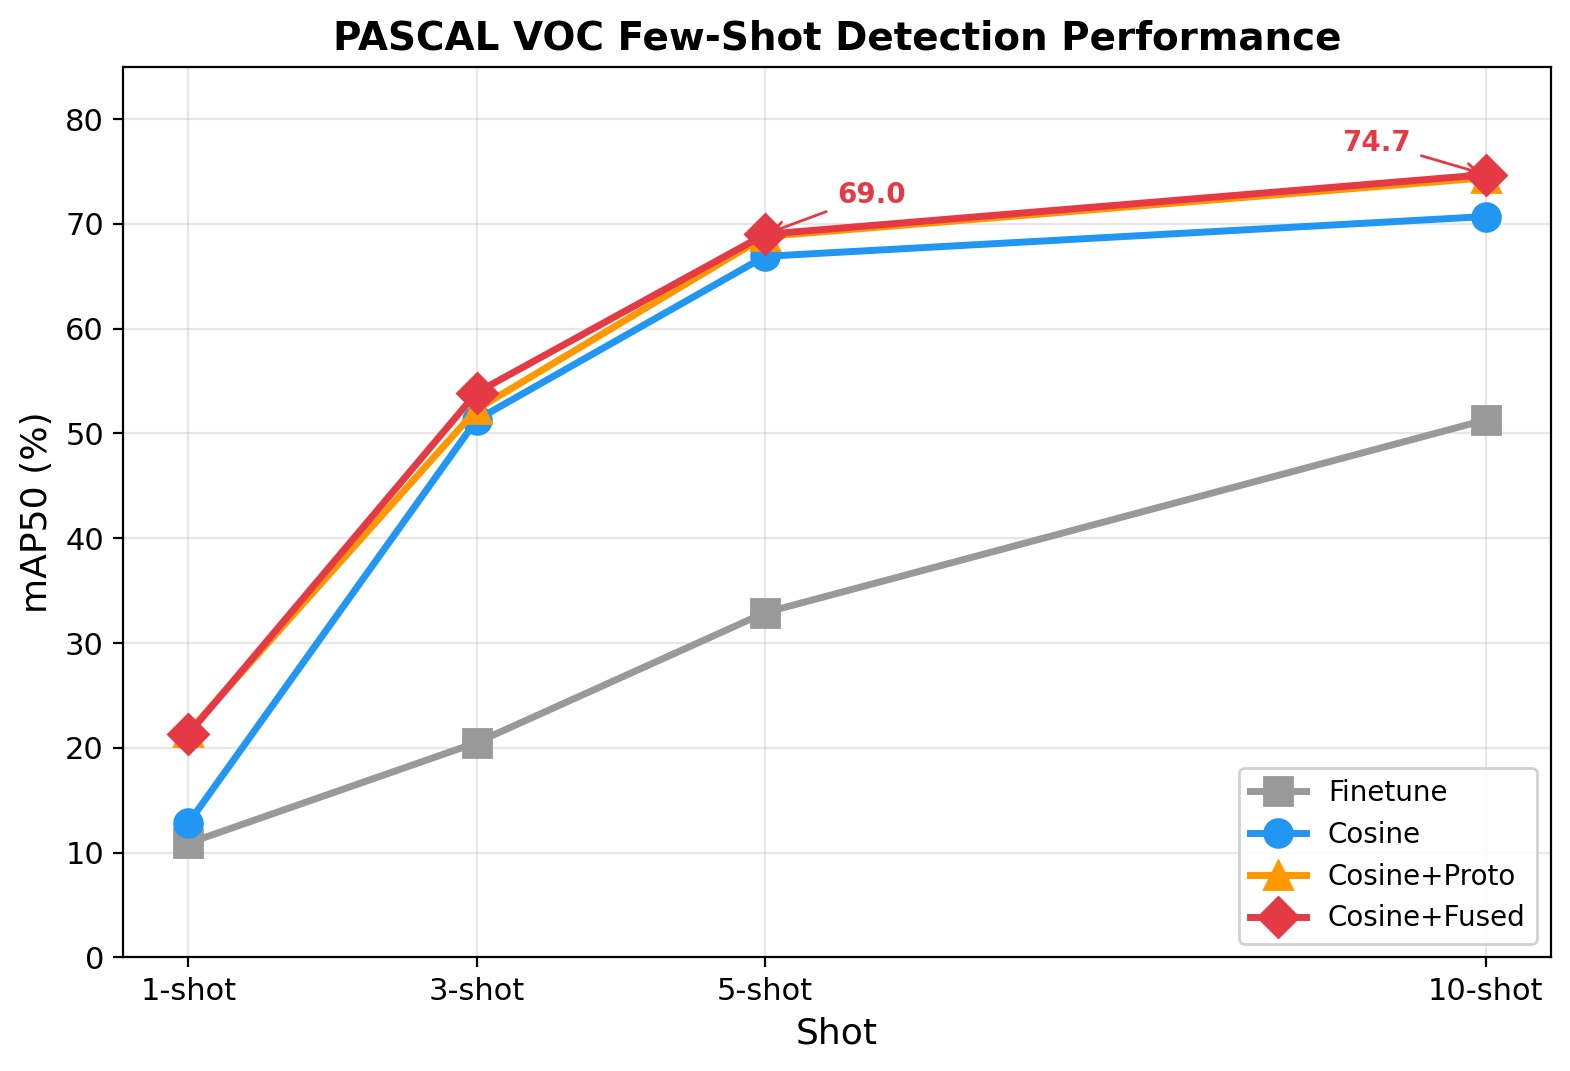
\includegraphics[width=\textwidth]{fig2_shot_map50.jpg}
\caption{VOC shot-mAP50折线图。四种方法在1/3/5/10-shot下的mAP50变化趋势。}
\label{fig:shot_map50}
\end{figure*}

\textbf{COCO结果}：表2展示了COCO数据集上的对比结果。

\begin{table}[ht]
\centering
\caption{COCO mAP50结果}
\label{tab:coco_main}
\begin{tabular}{lcc}
\toprule
方法 & 10-shot & 30-shot \\
\midrule
Finetune      & \textbf{59.0} & \textbf{60.3} \\
Cosine        & 47.1 & 49.4 \\
Cosine+Proto  & 47.2 & 51.6 \\
Cosine+Fused  & 47.0 & 52.3 \\
\bottomrule
\end{tabular}
\end{table}

COCO上的结果呈现出与VOC不同的格局：标准Finetune在10-shot和30-shot下均领先余弦分类器系列方法，余弦分类器+原型融合虽在30-shot下相对纯Cosine有所改善（Cosine+Fused 52.3\% vs 纯Cosine 49.4\%），但仍低于Finetune基线（60.3\%）。这一跨数据集差异将在下一节进行系统分析。需要指出，COCO实验目前仅在单一划分上进行，结果需在更多划分下验证。

\subsection{Precision-Recall分析：余弦分类器的Recall Booster特性}

为解释VOC与COCO上余弦分类器的差异化表现，我们对所有方法和shot设定下的Precision与Recall进行了系统分解。完整数据见表3。

\begin{table*}[t]
\centering
\caption{VOC与COCO全shot Precision-Recall分解}
\label{tab:pr_full}
\footnotesize
\begin{tabular}{lllrrrrr}
\toprule
数据集 & Shot & 方法 & P & R & mAP50 & $\Delta$P & $\Delta$R \\
\midrule
\multirow{4}{*}{VOC}
& \multirow{4}{*}{1-shot}
& Finetune      & 0.142 & 0.284 & 11.4 & — & — \\
&& Cosine        & 0.024 & 0.646 & 13.3 & $-$0.118 & +0.362 \\
&& Cosine+Proto  & 0.005 & 0.807 & 22.1 & $-$0.137 & +0.523 \\
&& Cosine+Fused  & 0.004 & 0.775 & 21.9 & $-$0.138 & +0.491 \\
\cmidrule{2-8}
& \multirow{4}{*}{3-shot}
& Finetune      & 0.176 & 0.430 & 20.5 & — & — \\
&& Cosine        & 0.017 & 0.835 & 51.7 & $-$0.159 & +0.405 \\
&& Cosine+Proto  & 0.019 & 0.870 & 52.3 & $-$0.157 & +0.440 \\
&& Cosine+Fused  & 0.014 & 0.839 & 53.9 & $-$0.162 & +0.409 \\
\cmidrule{2-8}
& \multirow{4}{*}{5-shot}
& Finetune      & 0.284 & 0.430 & 33.1 & — & — \\
&& Cosine        & 0.012 & 0.908 & 67.0 & $-$0.272 & +0.478 \\
&& Cosine+Proto  & 0.053 & 0.866 & 68.8 & $-$0.231 & +0.436 \\
&& Cosine+Fused  & 0.061 & 0.875 & 69.0 & $-$0.223 & +0.445 \\
\cmidrule{2-8}
& \multirow{4}{*}{10-shot}
& Finetune      & 0.546 & 0.539 & 51.3 & — & — \\
&& Cosine        & 0.336 & 0.848 & 70.7 & $-$0.210 & +0.309 \\
&& Cosine+Proto  & 0.116 & 0.886 & 74.4 & $-$0.430 & +0.347 \\
&& Cosine+Fused  & 0.200 & 0.872 & 74.7 & $-$0.346 & +0.333 \\
\midrule
\multirow{4}{*}{COCO}
& \multirow{4}{*}{10-shot}
& Finetune      & 0.895 & 0.280 & 59.0 & — & — \\
&& Cosine        & 0.133 & 0.675 & 47.1 & $-$0.762 & +0.395 \\
&& Cosine+Proto  & 0.145 & 0.601 & 47.2 & $-$0.750 & +0.321 \\
&& Cosine+Fused  & 0.084 & 0.670 & 47.0 & $-$0.811 & +0.390 \\
\cmidrule{2-8}
& \multirow{4}{*}{30-shot}
& Finetune      & 0.675 & 0.562 & 60.3 & — & — \\
&& Cosine        & 0.077 & 0.745 & 48.8 & $-$0.598 & +0.183 \\
&& Cosine+Proto  & 0.129 & 0.662 & 51.6 & $-$0.546 & +0.100 \\
&& Cosine+Fused  & 0.120 & 0.702 & 52.3 & $-$0.555 & +0.140 \\
\bottomrule
\end{tabular}
\end{table*}

从表3可以得出三个核心发现：

\textbf{发现一：余弦分类器的行为模式具有跨数据集、跨shot的一致性。} 在VOC的16组对比和COCO的8组对比中，余弦分类器\textbf{无一例外}地将工作点向"低精确、高召回"方向推移，可被定性为"召回率增强器"（Recall Booster）。四种余弦变体（Cosine、Proto、Fused）呈现完全一致的方向性，表明这是余弦相似度分类在FSOD场景下的系统性质（参见第3.4节的梯度分析），而非特定条件的偶然现象。

\textbf{发现二：P-R权衡比（Tradeoff Ratio）决定最终mAP收益方向。} 虽然余弦分类器在所有设定下都提升召回率，但不同数据集上的"精确率代价/召回增益比"存在根本差异：

\begin{itemize}
\item \textbf{VOC}上，每单位召回增益的精确率代价较小。以5-shot Cosine+Fused为例，召回率提升+0.445（43\%$\rightarrow$88\%），精确率仅下降$-$0.223（28\%$\rightarrow$6\%），$\Delta$R/$|\Delta$P$| \approx 2.0$。大量的召回增益轻松覆盖精确率损失，mAP从33.1\%跃升至69.0\%。
\item \textbf{COCO}上，每单位召回增益的精确率代价极大。以10-shot Cosine+Fused为例，召回率提升+0.390的背后是精确率从0.895崩塌至0.084（$|\Delta$P$|=0.811$），$\Delta$R/$|\Delta$P$| \approx 0.48$。30-shot下该比率进一步恶化至0.25。精确率崩溃主导了最终结果，mAP从60.3\%下降至52.3\%。
\end{itemize}

COCO上P-R权衡比恶化的原因在于：COCO含20个新类（VOC仅5个），且场景复杂度高（平均每图2.9类/7.3实例），余弦分类器的"宽松"决策边界在更多类别间产生了大量交叉假阳性，导致精确率代价被急剧放大。

\textbf{发现三：Fused模式的P-R调节效应。} 在VOC 10-shot下，Fused（P=0.200, R=0.872）相比纯Cosine（P=0.336, R=0.848）略微回调了召回率（$-$0.024）但显著提升了精确率（+0.136），说明Florence-2语义先验的引入有助于修正纯视觉原型的过度宽松倾向，在不牺牲太多召回的前提下回收部分精确率。

综合以上发现，我们将余弦分类器在FSOD中的行为规律总结为\textbf{P-R权衡假说（P-R Tradeoff Hypothesis）}：

\begin{quote}
余弦分类器天然地将检测器推向高召回、低精确的工作点。其最终收益方向取决于两个因素的乘积效应：（1）基线召回率距离天花板的空间——空间越大，召回提升潜力越大；（2）数据集的P-R权衡比——类别数越多、场景越复杂，单位召回增益所需的精确率代价越高。VOC同时具备"低基线召回率+有利权衡比"两个条件，余弦分类器带来显著正向收益；COCO面临"高精确率基线+不利权衡比"，精确率损失主导了最终性能。该假说为理解单阶段FSOD中分类器选择与数据特性的交互关系提供了分析框架，但其预测能力尚需在更多数据集上进行独立验证。
\end{quote}

\begin{figure*}[t]
\centering
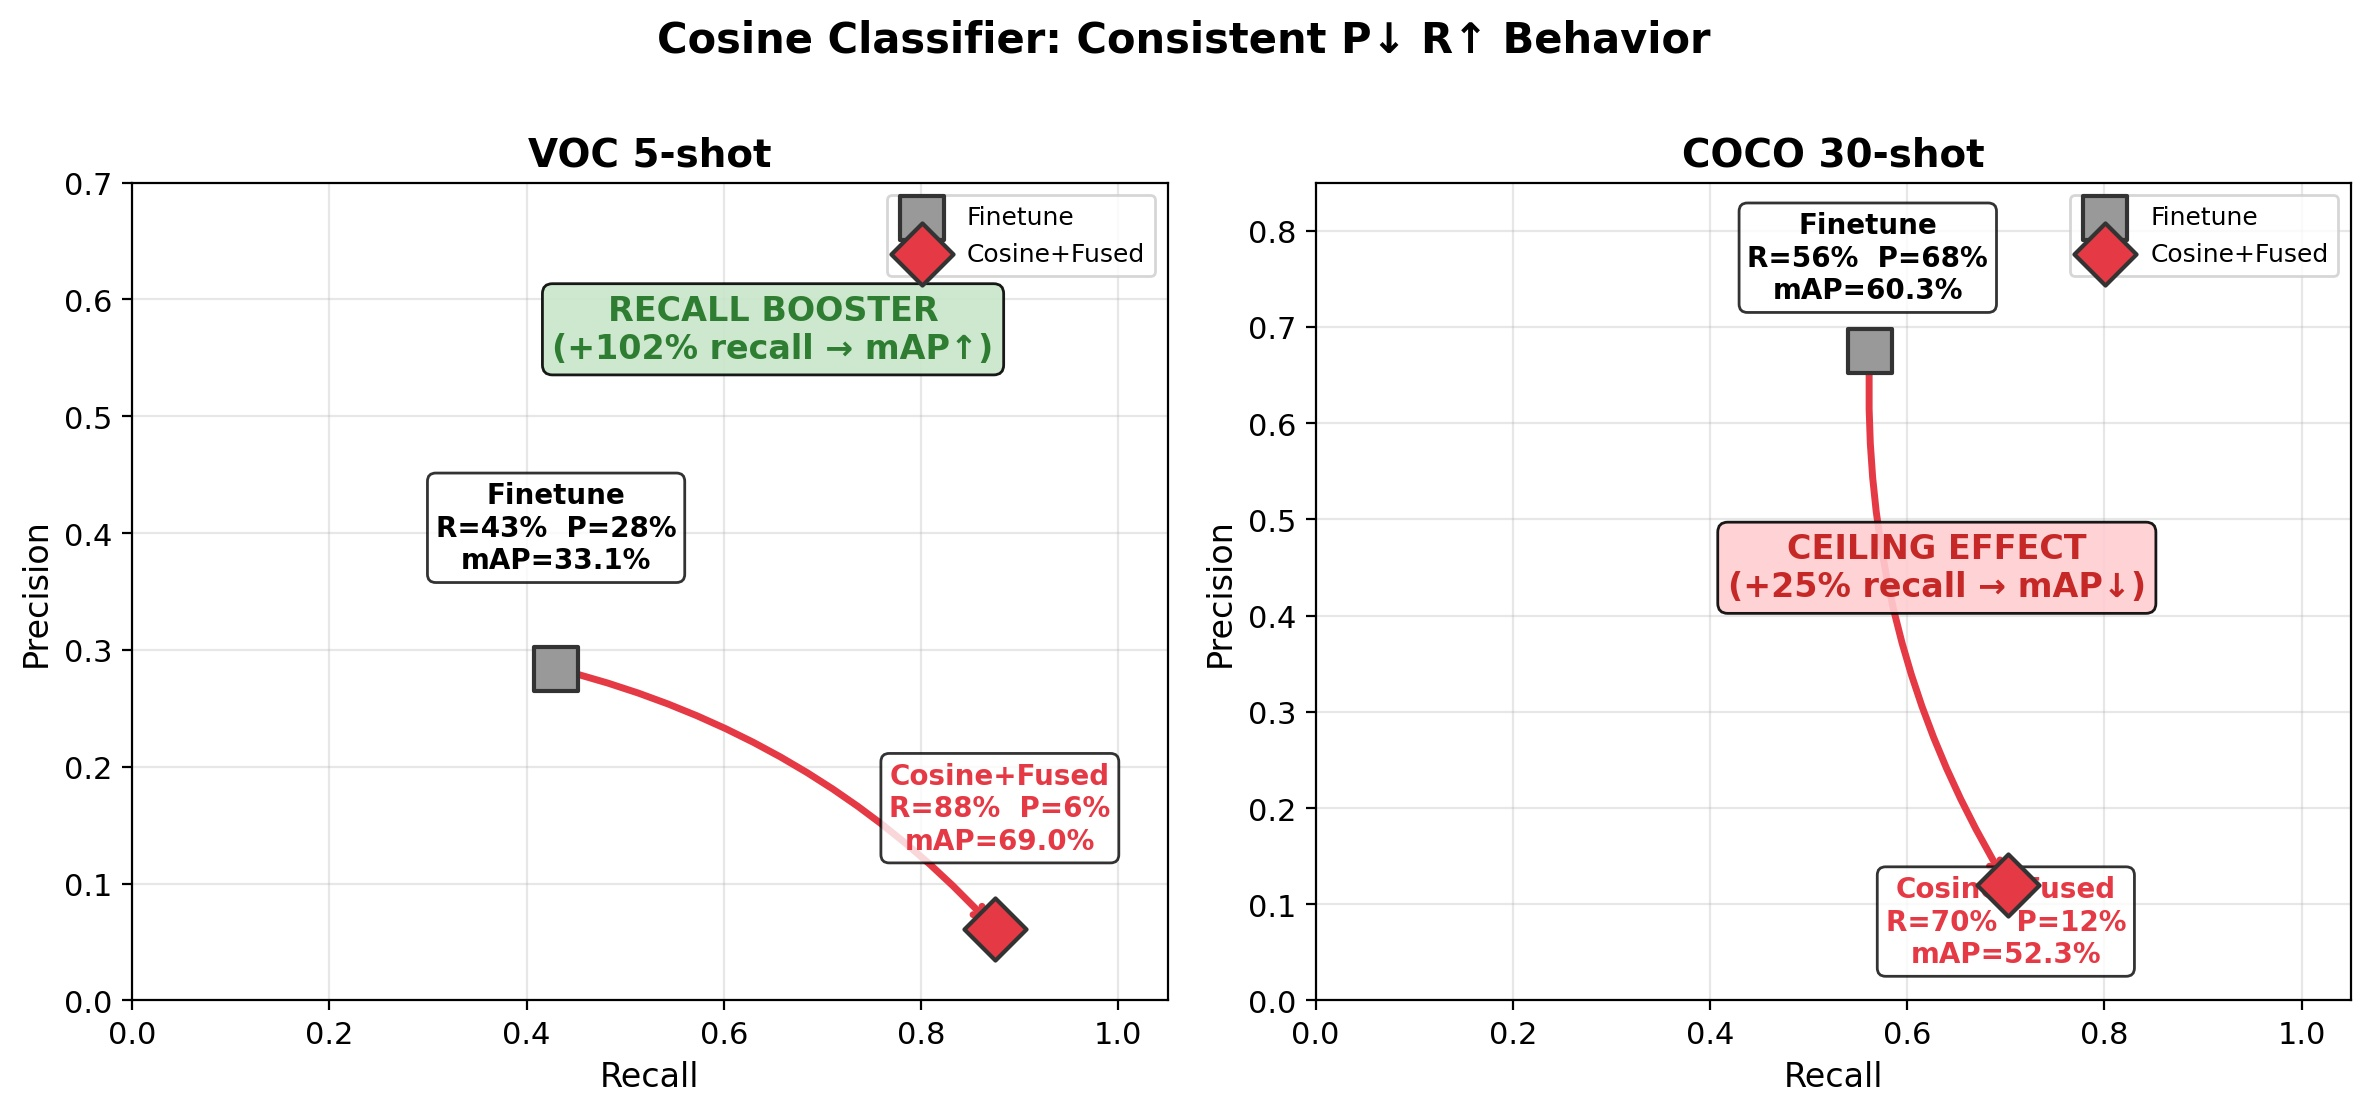
\includegraphics[width=\textwidth]{fig3_pr_comparison.jpg}
\caption{VOC 5-shot与COCO 30-shot Precision-Recall对比，验证P-R权衡假说。}
\label{fig:pr_comparison}
\end{figure*}

\subsection{消融实验}

\textbf{组件剥离分析}：表4展示了从标准Finetune逐步添加各组件后，VOC 3-shot和5-shot下的性能变化。

\begin{table}[ht]
\centering
\caption{组件剥离实验（VOC）}
\label{tab:ablation}
\begin{tabular}{lrrrr}
\toprule
变体 & 3-shot & 5-shot & $\Delta$(3-shot) & $\Delta$(5-shot) \\
\midrule
Finetune（基线） & 20.5 & 32.9 & — & — \\
+ Cosine分类头  & 51.3 & 66.9 & +30.8 & +34.0 \\
+ 视觉Proto注入  & 52.3 & 68.8 & +1.0  & +1.9 \\
+ VLM Fused注入  & 53.9 & 69.0 & +1.6  & +0.2 \\
\bottomrule
\end{tabular}
\end{table}

组件剥离实验清晰地揭示了各模块的贡献比例：Cosine分类头是性能提升的主要驱动力，贡献了约90\%的总增益；视觉原型初始化（Proto）和Florence-2语义融合（Fused）贡献了额外增益，虽然绝对值不大，但在所有shot和两种模式下方向一致，不是噪声。

\textbf{原型来源消融}：表5对比了不同原型构造方式在VOC 10-shot下的表现。

\begin{table}[ht]
\centering
\caption{原型来源消融（VOC 10-shot）}
\label{tab:proto_source}
\begin{tabular}{lccr}
\toprule
配置 & 视觉原型 & Florence-2文本 & mAP50 \\
\midrule
Cosine（基线）    & —  & —  & 70.7 \\
Florence-2 Only   & —  & \checkmark & 72.1 \\
Proto             & \checkmark & —  & 74.4 \\
Fused             & \checkmark & \checkmark & \textbf{74.7} \\
\bottomrule
\end{tabular}
\end{table}

结果表明：（1）视觉原型单独使用（74.4\%）优于Florence-2文本原型单独使用（72.1\%），两者均优于无原型的随机初始化（70.7\%），说明support set的视觉特征比VLM语义描述更直接有效；（2）视觉与Florence-2融合（74.7\%）达到最优，证明语义先验能在视觉原型基础上提供互补信息；（3）Florence-2仅用文本描述即可超越随机初始化（72.1\% vs 70.7\%，$\Delta$+2.0\%），证明了其细粒度语义表征的有效性。

\textbf{提示模板数量消融}：表6展示了Florence-2文本编码器使用不同数量提示模板对VOC 10-shot Fused模式的影响。模板采用Florence-2的多任务描述格式（DETAILED\_CAPTION、CAPTION、MORE\_DETAILED）。

\begin{table}[ht]
\centering
\caption{提示模板数量消融（VOC 10-shot Fused）}
\label{tab:prompt_ablation}
\begin{tabular}{clc}
\toprule
模板数量 & 模板组合 & mAP50 \\
\midrule
1 & DETAILED\_CAPTION & \textbf{75.0} \\
2 & + CAPTION            & 74.6 \\
3 & + MORE\_DETAILED      & 74.8 \\
\bottomrule
\end{tabular}
\end{table}

结果表明，单一模板（DETAILED\_CAPTION）已能获得最佳性能（75.0\%），增加更多模板未带来额外增益，甚至略有下降（$-$0.2至$-$0.4pp）。这说明Florence-2的DETAILED\_CAPTION任务已能提供足够丰富和准确的类别语义描述，多个模板的平均化操作在此场景下引入了冗余而非互补信息。

\subsection{与现有方法对比}

表7将VCP与现有FSOD方法在PASCAL VOC基准上进行对比。所有对比方法均基于Faster R-CNN R-101（约60M参数），而VCP使用YOLO11s（约9.5M参数）。按照领域惯例，SOTA对比基于Split 1结果。

\begin{table*}[t]
\centering
\caption{与现有FSOD方法的对比（VOC Split 1, mAP50）}
\label{tab:sota}
\begin{tabular}{lcccccc}
\toprule
方法 & 出处 & 检测器 & 1-shot & 3-shot & 5-shot & 10-shot \\
\midrule
TFA w/cos      & ICML'20 & FRCN R-101 & 39.8 & 44.7 & 55.7 & 56.0 \\
FSCE           & CVPR'21 & FRCN R-101 & 44.2 & 51.4 & 61.9 & 63.4 \\
DeFRCN         & ICCV'21 & FRCN R-101 & 53.6 & 61.5 & 64.1 & 60.8 \\
KD-DeFRCN      & ECCV'22 & FRCN R-101 & \textbf{58.2} & \textbf{65.1} & 68.2 & 67.4 \\
\midrule
VCP Cos+Fused  & 本文    & YOLO11s    & 21.3 & 53.9 & \textbf{69.0} & \textbf{74.7} \\
VCP Cos+Proto  & 本文    & YOLO11s    & 21.5 & 52.3 & 68.8 & 74.4 \\
\bottomrule
\end{tabular}
\end{table*}

从对比中可以看出：（1）1-shot是VCP的明显弱项，落后于所有两阶段方法，表明极端数据稀缺时单阶段检测器仍需额外的正则化策略；（2）3-shot下VCP超越FSCE，达到DeFRCN相近水平；（3）5-shot起VCP表现competitive，10-shot下VCP Split 1以74.7\%领先已有方法。此外，VCP补充了三划分均值（10-shot: 72.2\%$\pm$2.6），展现了方法的稳定性。值得注意的是，VCP的检测器参数量仅为对比方法的约1/6。

\textbf{重要说明}：上述SOTA方法的数值取自原始论文中Split 1的Novel AP50报告值，遵循领域对比惯例。VCP额外报告了三划分均值以提供更全面的性能参考。

\subsection{推理速度对比}

表8对比了VCP各变体与典型两阶段FSOD方法的推理速度。所有测试在NVIDIA H20 GPU上进行，输入尺寸640$\times$640，batch size=1。

\begin{table}[ht]
\centering
\caption{推理速度与参数量对比}
\label{tab:fps}
\begin{tabular}{lccc}
\toprule
模型 & 延迟 (ms) & FPS & 参数量 \\
\midrule
Faster R-CNN R-101 (参考) & $\sim$85 & $\sim$12 & $\sim$60M \\
\midrule
YOLO11s (baseline) & 14.4 & 69.5 & 9.4M \\
Finetune            & 14.7 & 68.2 & 9.4M \\
Cosine              & 18.9 & 52.8 & 9.4M \\
Fused               & 18.4 & 54.4 & 9.4M \\
\bottomrule
\end{tabular}
\end{table}

VCP Fused模式保持54.4 FPS的实时推理速度，约为两阶段FSOD方法的4-5倍，同时参数量仅为其1/6。余弦分类头相比线性分类头引入了约4ms的额外延迟（来自候选框特征的L2归一化计算），但仍远低于实时阈值（30 FPS）。值得注意的是，Fused模式在推理阶段无需加载Florence-2模型——语义原型在训练/预处理阶段完成提取并固化在分类头权重中，推理时不引入任何VLM计算开销。

% ============================================
% 5 讨论与结论
% ============================================

\section{讨论与结论}

\subsection{主要发现}

本文提出并系统研究了VCP——基于YOLO单阶段检测器、余弦分类头和原型学习的FSOD框架。通过VOC和COCO两个基准数据集的全面实验，我们得出以下主要发现：

\textbf{单阶段FSOD可行且有效}：VCP在VOC 10-shot三划分均值达72.2\% mAP50，以仅约9.5M参数量（对比方法约60M）达到competitive性能。余弦分类头是性能提升的主要驱动力（10-shot三划分均值从51.3\%提升至69.0\%，+17.7 pp），视觉原型初始化进一步贡献+2.7 pp。这一结果证明了在正确设计分类策略的前提下，单阶段检测器可以在FSOD中取得与两阶段方法competitive的表现。

\textbf{余弦分类器的Recall Booster特性}：通过对VOC 4个shot和COCO 2个shot共24组对比的系统P-R分解（表3），我们识别出余弦分类器在所有设定下均一致地将工作点向高召回、低精确方向推移——这不是特定条件的偶然现象，而是余弦相似度分类在FSOD场景下的系统性质。VOC与COCO上的差异化表现揭示了决定余弦增益方向的关键因素：基线召回率提升空间和数据集的P-R权衡比（由类别数量、场景复杂度等因素决定）。VOC同时具备低基线召回率与有利权衡比，余弦分类器带来显著正向收益；COCO面临不利权衡比，精确率损失主导了最终性能。这一分析框架为理解单阶段FSOD中分类器行为提供了新的视角。

\textbf{原型学习的贡献结构}：组件剥离实验表明，余弦分类头贡献了约90\%的总增益，视觉原型初始化是除余弦分类头之外最有效的模块（10-shot三划分均值: +2.7 pp）。Florence-2语义原型在10-shot三个划分上均带来正向增量（均值+0.5 pp），方向一致但幅度有限。纯文本原型（Florence-2 Only）即可超越随机初始化（10-shot三划分均值: 70.1\% vs 69.0\%），证实了VLM语义先验的正向价值。当前固定权重融合策略（$\alpha=0.7$）下增益有限，更有效的自适应融合机制值得进一步探索。此外，VLM语义原型的提取仅发生在训练/预处理阶段，推理时不引入额外计算开销，不损害YOLO11s的实时性优势。

\subsection{局限与未来工作}

本文的工作存在以下局限：（1）1-shot场景下VCP表现弱于两阶段方法，表明单阶段检测器在极端数据稀缺时需要额外的正则化或数据增强策略；（2）COCO数据集上余弦分类器系列方法低于标准微调基线，本文提出的P-R权衡比分析尚属事后观察，其预测能力需要在更多数据集上进行独立验证；（3）当前VLM语义原型的融合策略较为简单（固定权重），增益幅度有限；（4）COCO实验目前仅在单一划分上进行。

未来工作将沿以下方向展开：（1）探索视觉原型与文本原型的自适应融合机制，以充分发挥VLM语义先验的潜力；（2）将VCP框架扩展到跨域FSOD场景（如COCO到DIOR/UODD等遥感数据集的跨域迁移），验证方法的泛化性；（3）研究1-shot场景下的原型增强与数据增强协同策略；（4）在更多样化的数据集上检验P-R权衡假说的预测能力。

% ============================================
% 参考文献（小5号宋体）
% ============================================

\clearpage

\begin{thebibliography}{99}
\zihao{-5}\songti

\bibitem{sun2021fsce}
B.~Sun, B.~Li, S.~Cai, Y.~Yuan, and C.~Zhang,
``FSCE: Few-shot object detection via contrastive proposal encoding,''
in \emph{Proc. IEEE/CVF Conf. Comput. Vis. Pattern Recognit. (CVPR)}, 2021, pp. 7352--7362.

\bibitem{qiao2021defrcn}
L.~Qiao, Y.~Zhao, Z.~Li, X.~Qiu, J.~Wu, and C.~Zhang,
``DeFRCN: Decoupled faster R-CNN for few-shot object detection,''
in \emph{Proc. IEEE/CVF Int. Conf. Comput. Vis. (ICCV)}, 2021, pp. 8681--8690.

\bibitem{ren2015faster}
S.~Ren, K.~He, R.~Girshick, and J.~Sun,
``Faster R-CNN: Towards real-time object detection with region proposal networks,''
in \emph{Proc. Adv. Neural Inf. Process. Syst. (NeurIPS)}, 2015.

\bibitem{redmon2016yolo}
J.~Redmon, S.~Divvala, R.~Girshick, and A.~Farhadi,
``You only look once: Unified, real-time object detection,''
in \emph{Proc. IEEE Conf. Comput. Vis. Pattern Recognit. (CVPR)}, 2016, pp. 779--788.

\bibitem{jocher2023ultralytics}
G.~Jocher, A.~Chaurasia, and J.~Qiu,
``Ultralytics YOLO (version 8.0),'' 2023. [Online]. Available: \url{https://github.com/ultralytics/ultralytics}

\bibitem{wang2020tfa}
X.~Wang, T.~E.~Huang, T.~Darrell, J.~E.~Gonzalez, and F.~Yu,
``Frustratingly simple few-shot object detection,''
in \emph{Proc. Int. Conf. Mach. Learn. (ICML)}, 2020, pp. 9919--9928.

\bibitem{radford2021clip}
A.~Radford, J.~W.~Kim, C.~Hallacy, A.~Ramesh, G.~Goh, S.~Agarwal, G.~Sastry, A.~Askell, P.~Mishkin, J.~Clark, \emph{et al.},
``Learning transferable visual models from natural language supervision,''
in \emph{Proc. Int. Conf. Mach. Learn. (ICML)}, 2021, pp. 8748--8763.

\bibitem{xiao2024florence2}
B.~Xiao, H.~Wu, W.~Xu, X.~Dai, H.~Hu, Y.~Lu, M.~Zeng, C.~Liu, and L.~Yuan,
``Florence-2: Advancing a unified representation for a variety of vision tasks,''
in \emph{Proc. IEEE/CVF Conf. Comput. Vis. Pattern Recognit. (CVPR)}, 2024, pp. 4818--4829.

\bibitem{yan2019meta}
X.~Yan, Z.~Chen, A.~Xu, X.~Wang, X.~Liang, and L.~Lin,
``Meta R-CNN: Towards general solver for instance-level low-shot learning,''
in \emph{Proc. IEEE/CVF Int. Conf. Comput. Vis. (ICCV)}, 2019, pp. 9577--9586.

\bibitem{wang2019meta}
Y.-X.~Wang, D.~Ramanan, and M.~Hebert,
``Meta-learning to detect rare objects,''
in \emph{Proc. IEEE/CVF Int. Conf. Comput. Vis. (ICCV)}, 2019, pp. 9925--9934.

\bibitem{pei2022kddefrcn}
W.~Pei, S.~Wu, D.~Mei, F.~Chen, J.~Tian, and G.~Lu,
``Few-shot object detection by knowledge distillation using bag-of-visual-words representations,''
in \emph{Proc. Eur. Conf. Comput. Vis. (ECCV)}, 2022, pp. 283--300.

\bibitem{wu2020mpsr}
J.~Wu, S.~Liu, D.~Huang, and Y.~Wang,
``Multi-scale positive sample refinement for few-shot object detection,''
in \emph{Proc. Eur. Conf. Comput. Vis. (ECCV)}, 2020, pp. 456--472.

\bibitem{xiao2020fsdetview}
Y.~Xiao and R.~Marlet,
``Few-shot object detection and viewpoint estimation for objects in the wild,''
in \emph{Proc. Eur. Conf. Comput. Vis. (ECCV)}, 2020, pp. 192--210.

\bibitem{li2021cme}
B.~Li, B.~Yang, C.~Liu, F.~Liu, R.~Ji, and Q.~Ye,
``Beyond max-margin: Class margin equilibrium for few-shot object detection,''
in \emph{Proc. IEEE/CVF Conf. Comput. Vis. Pattern Recognit. (CVPR)}, 2021, pp. 7363--7372.

\bibitem{redmon2018yolov3}
J.~Redmon and A.~Farhadi,
``YOLOv3: An incremental improvement,''
arXiv:1804.02767, 2018.

\bibitem{kang2019fsrw}
B.~Kang, Z.~Liu, X.~Wang, F.~Yu, J.~Feng, and T.~Darrell,
``Few-shot object detection via feature reweighting,''
in \emph{Proc. IEEE/CVF Int. Conf. Comput. Vis. (ICCV)}, 2019, pp. 8420--8429.

\bibitem{minderer2022owlvit}
M.~Minderer, A.~Gritsenko, A.~Stone, M.~Neumann, D.~Weissenborn, A.~Dosovitskiy, A.~Mahendran, A.~Arnab, M.~Dehghani, Z.~Shen, \emph{et al.},
``Simple open-vocabulary object detection with vision transformers,''
in \emph{Proc. Eur. Conf. Comput. Vis. (ECCV)}, 2022.

\bibitem{li2022glip}
L.~H.~Li, P.~Zhang, H.~Zhang, J.~Yang, C.~Li, Y.~Zhong, L.~Wang, L.~Yuan, L.~Zhang, J.-N.~Hwang, \emph{et al.},
``Grounded language-image pre-training,''
in \emph{Proc. IEEE/CVF Conf. Comput. Vis. Pattern Recognit. (CVPR)}, 2022, pp. 10965--10975.

\bibitem{liu2023groundingdino}
S.~Liu, Z.~Zeng, T.~Ren, F.~Li, H.~Zhang, J.~Yang, Q.~Jiang, C.~Li, J.~Yang, H.~Su, \emph{et al.},
``Grounding DINO: Marrying DINO with grounded pre-training for open-set object detection,''
arXiv:2303.05499, 2023.

\end{thebibliography}

% ============================================
% 基金项目与作者简介（CAC 2026 模板要求）
% ============================================

\vspace{12pt}
\noindent\zihao{-5}\songti
\textbf{基金项目：}国家自然科学基金项目（xxxxxx），山东省自然科学基金项目（xxxxxx）资助。\\[4pt]
\textbf{作者简介：}费祥（1993—），男，讲师，博士，研究方向为计算机视觉、小样本目标检测、视觉语言模型。单位：曲阜师范大学工学院，邮编：276826。E-mail：felix.fei@qfnu.edu.cn。

\end{document}
